% source-sha256: 26f018f2a69c7fc401c60e9fc61c8b7d56ead1111ad197706a2ed3ef7f28ac6c
% Options for packages loaded elsewhere
\PassOptionsToPackage{unicode}{hyperref}
\PassOptionsToPackage{hyphens}{url}
\documentclass[
]{article}
\usepackage{xcolor}
\usepackage[letterpaper,margin=1in]{geometry}
\usepackage{amsmath,amssymb}
\setcounter{secnumdepth}{-\maxdimen} % remove section numbering
\usepackage{iftex}
\ifPDFTeX
  \usepackage[T1]{fontenc}
  \usepackage[utf8]{inputenc}
  \usepackage{textcomp} % provide euro and other symbols
\else % if luatex or xetex
  \usepackage{unicode-math} % this also loads fontspec
  \defaultfontfeatures{Scale=MatchLowercase}
  \defaultfontfeatures[\rmfamily]{Ligatures=TeX,Scale=1}
\fi
\usepackage{lmodern}
\ifPDFTeX\else
  % xetex/luatex font selection
\fi
% Use upquote if available, for straight quotes in verbatim environments
\IfFileExists{upquote.sty}{\usepackage{upquote}}{}
\IfFileExists{microtype.sty}{% use microtype if available
  \usepackage[]{microtype}
  \UseMicrotypeSet[protrusion]{basicmath} % disable protrusion for tt fonts
}{}
\makeatletter
\@ifundefined{KOMAClassName}{% if non-KOMA class
  \IfFileExists{parskip.sty}{%
    \usepackage{parskip}
  }{% else
    \setlength{\parindent}{0pt}
    \setlength{\parskip}{6pt plus 2pt minus 1pt}}
}{% if KOMA class
  \KOMAoptions{parskip=half}}
\makeatother
\usepackage{longtable,booktabs,array}
\usepackage{caption}
\captionsetup[table]{skip=6pt}
\newcounter{none} % for unnumbered tables
\usepackage{calc} % for calculating minipage widths
% Correct order of tables after \paragraph or \subparagraph
\usepackage{etoolbox}
\makeatletter
\patchcmd\longtable{\par}{\if@noskipsec\mbox{}\fi\par}{}{}
\makeatother
% Allow footnotes in longtable head/foot
\IfFileExists{footnotehyper.sty}{\usepackage{footnotehyper}}{\usepackage{footnote}}
\makesavenoteenv{longtable}
\setlength{\emergencystretch}{3em} % prevent overfull lines
\providecommand{\tightlist}{%
  \setlength{\itemsep}{0pt}\setlength{\parskip}{0pt}}
% Release-document layout safeguards injected by scripts/generate_docs.sh.
\usepackage{fvextra}
\fvset{breaklines=true,breakanywhere=true,fontsize=\small}
\RecustomVerbatimEnvironment{verbatim}{Verbatim}{breaklines=true,breakanywhere=true,fontsize=\small}
\setlength{\emergencystretch}{3em}
\AtBeginDocument{\sloppy}
% Workflow-figure support: mermaid blocks in the canonical Markdown are mapped
% to hand-authored TikZ figures by scripts/pandoc_bounded_tables.lua.
\usepackage{tikz}
\usetikzlibrary{shapes.geometric,arrows.meta,positioning,fit,backgrounds,calc}
\definecolor{bdiStep}{HTML}{EAF2FB}
\definecolor{bdiEdge}{HTML}{365F91}
\definecolor{bdiText}{HTML}{17253A}
\definecolor{bdiGate}{HTML}{FFF5D6}
\definecolor{bdiGateEdge}{HTML}{9B6B00}
\definecolor{bdiOpt}{HTML}{F0EAF7}
\definecolor{bdiOptEdge}{HTML}{5B3E86}
\definecolor{bdiOut}{HTML}{E6F4EA}
\definecolor{bdiOutEdge}{HTML}{1E6B3A}
\tikzset{
  bdi/.style={draw=bdiEdge,line width=1pt,fill=bdiStep,text=bdiText,rounded corners=3pt,
              align=center,inner sep=4pt,font=\scriptsize\sffamily},
  bdigate/.style={bdi,draw=bdiGateEdge,fill=bdiGate},
  bdiopt/.style={bdi,draw=bdiOptEdge,fill=bdiOpt,dashed},
  bdiout/.style={bdi,draw=bdiOutEdge,fill=bdiOut},
  bdiflow/.style={-{Stealth[length=2mm]},draw=bdiEdge,line width=0.9pt},
  bdiback/.style={bdiflow,dashed},
  bdilbl/.style={font=\tiny\sffamily,text=bdiText,inner sep=1.5pt,fill=white},
}
\usepackage{bookmark}
\IfFileExists{xurl.sty}{\usepackage{xurl}}{} % add URL line breaks if available
\urlstyle{same}
% fallback for those not using the hyperref driver hyperxmp:
\makeatletter
\@ifundefined{xmpquote}{\newcommand{\xmpquote}[1]{#1}}{}
\makeatother
\hypersetup{
  hidelinks,
  pdfcreator={LaTeX via pandoc}}

\author{}
\date{}

\begin{document}

\section{How the document process
works}\label{how-the-document-process-works}

\subsection{What this guide explains}\label{what-this-guide-explains}

This plain-language guide explains what happens to a document delivery,
what the system can establish from evidence, and where a client decision
is still needed. It is a companion to the Client Overview and Client
User Guide, and it is written to be read on its own: every stage below
states what the stage does, how it does it, and what it produces.

The central promise is simple: the system preserves what was supplied,
explains how it reached each proposed conclusion, and leaves uncertainty
visible. It does not silently replace a source value, invent an
accounting record, or treat an AI response as approval.

\subsection{Three words that carry the whole
process}\label{three-words-that-carry-the-whole-process}

Almost every question about this system is answered by knowing which of
three states a piece of information is in. The states never blur
together, and nothing moves between them by itself.

{\def\LTcaptype{none} % do not increment counter
\begin{longtable}[]{@{}
  >{\raggedright\arraybackslash}p{(\linewidth - 4\tabcolsep) * \real{0.3333}}
  >{\raggedright\arraybackslash}p{(\linewidth - 4\tabcolsep) * \real{0.3333}}
  >{\raggedright\arraybackslash}p{(\linewidth - 4\tabcolsep) * \real{0.3333}}@{}}
\toprule\noalign{}
\begin{minipage}[b]{\linewidth}\raggedright
State
\end{minipage} & \begin{minipage}[b]{\linewidth}\raggedright
What it means
\end{minipage} & \begin{minipage}[b]{\linewidth}\raggedright
What can change it
\end{minipage} \\
\midrule\noalign{}
\endhead
\bottomrule\noalign{}
\endlastfoot
\textbf{Evidence} & Something that was actually supplied --- a source
page, a returned workbook, a ledger export. & Nothing. Evidence is
retained unchanged, forever. \\
\textbf{Proposal} & Something the system worked out --- an extracted
value, a match, an AI-suggested link, a grouping. & Review. A proposal
is never a fact just because it looks confident. \\
\textbf{Authorized fact} & A proposal an operator explicitly approved,
applied as an append-only amendment. & Only a further authorized
amendment, which is also appended. \\
\end{longtable}
}

\begin{figure}[htbp]
\centering
\resizebox{\ifdim\width>\textwidth\textwidth\else\width\fi}{!}{%
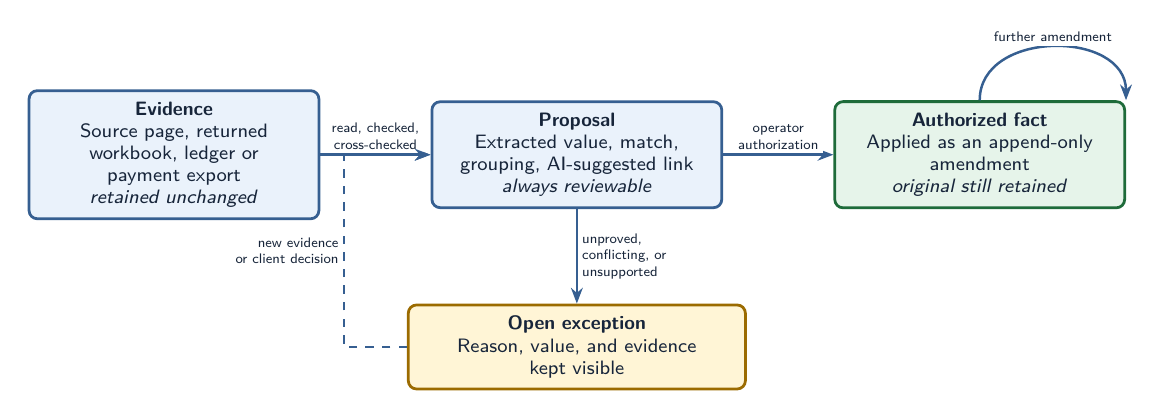
\begin{tikzpicture}[node distance=8mm and 14mm]
  \node[bdi,text width=34mm] (E) {\textbf{Evidence}\\Source page, returned\\workbook, ledger or\\payment export\\\emph{retained unchanged}};
  \node[bdi,text width=34mm,right=of E] (P) {\textbf{Proposal}\\Extracted value, match,\\grouping, AI-suggested link\\\emph{always reviewable}};
  \node[bdiout,text width=34mm,right=of P] (A) {\textbf{Authorized fact}\\Applied as an append-only\\amendment\\\emph{original still retained}};
  \node[bdigate,text width=40mm,below=12mm of P] (X) {\textbf{Open exception}\\Reason, value, and evidence\\kept visible};

  \draw[bdiflow] (E)--node[bdilbl,above,align=center]{read, checked,\\cross-checked}(P);
  \draw[bdiflow] (P)--node[bdilbl,above,align=center]{operator\\authorization}(A);
  \draw[bdiflow] (P)--node[bdilbl,right,align=left]{unproved,\\conflicting, or\\unsupported}(X);
  \draw[bdiback] (X.west) -- ++(-8mm,0) |- node[bdilbl,pos=0.25,left,align=right]{new evidence\\or client decision} (P.west);
  \draw[bdiflow] (A.north) .. controls +(0,9mm) and +(0,9mm) .. node[bdilbl,above]{further amendment} (A.north east);
\end{tikzpicture}
}
\caption{The three states of any value in the system. A proposal only becomes an authorized fact through explicit operator authorization, and the original reading is retained either way.}
\end{figure}

A confidence score, an agreement between two readers, and an AI
explanation are all just descriptions of a proposal. None of them
performs the authorization step.

\subsection{The workflow at a glance}\label{the-workflow-at-a-glance}

Read the solid spine from top to bottom: stages 1 to 6 and 8 to 10 are
deterministic, they run in that order, and they are the only path that
can clear a control. Stage 7, drawn to the side in dashes, is the
optional AI layer. It can add proposals and questions, but it never
clears a control and never writes a value on its own. The dashed arrow
returning from stage 9 to stage 3 is the rerun loop: once an authorized
change is applied, every stage it could affect runs again, so a
correction can never leave an earlier check reported against superseded
data.

\begin{figure}[htbp]
\centering
\resizebox{\ifdim\width>\textwidth\textwidth\else\width\fi}{!}{%
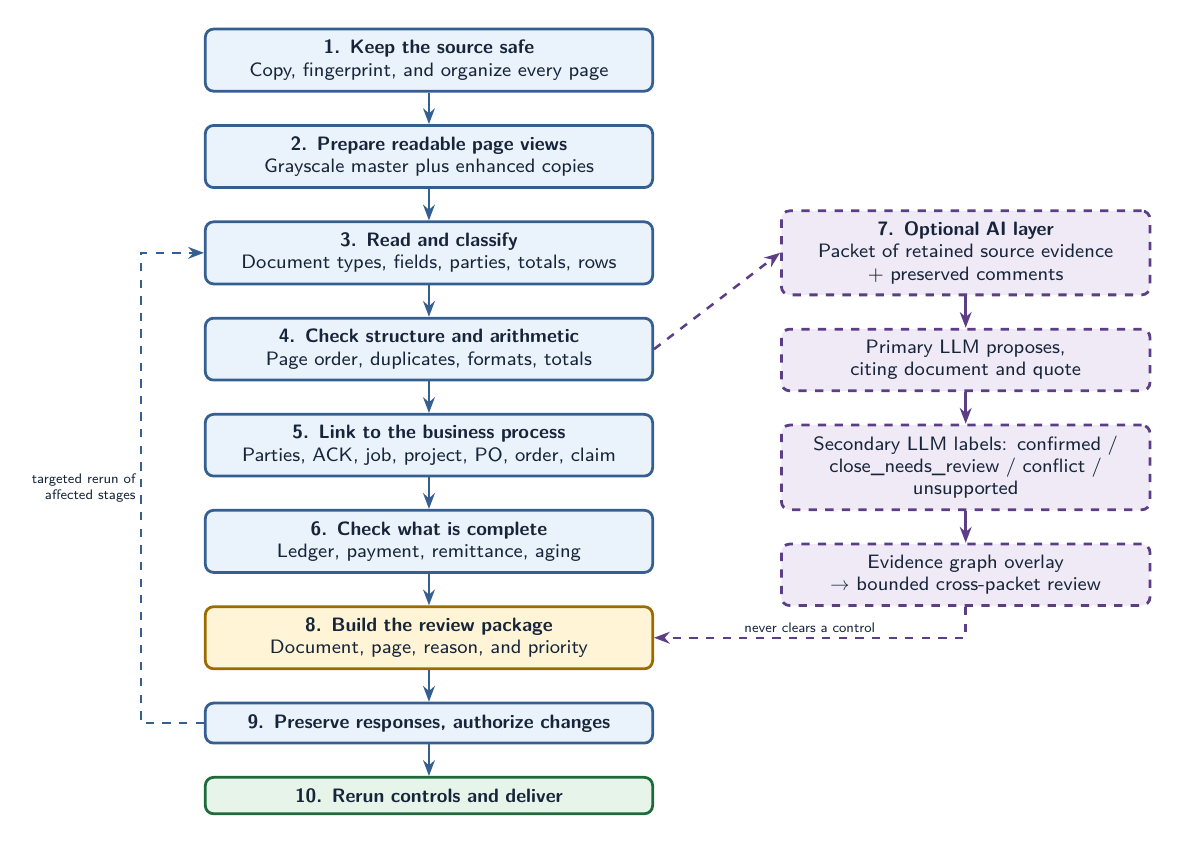
\begin{tikzpicture}[node distance=4mm and 10mm]
  \node[bdi,text width=54mm] (S1) {\textbf{1. Keep the source safe}\\Copy, fingerprint, and organize every page};
  \node[bdi,text width=54mm,below=of S1] (S2) {\textbf{2. Prepare readable page views}\\Grayscale master plus enhanced copies};
  \node[bdi,text width=54mm,below=of S2] (S3) {\textbf{3. Read and classify}\\Document types, fields, parties, totals, rows};
  \node[bdi,text width=54mm,below=of S3] (S4) {\textbf{4. Check structure and arithmetic}\\Page order, duplicates, formats, totals};
  \node[bdi,text width=54mm,below=of S4] (S5) {\textbf{5. Link to the business process}\\Parties, ACK, job, project, PO, order, claim};
  \node[bdi,text width=54mm,below=of S5] (S6) {\textbf{6. Check what is complete}\\Ledger, payment, remittance, aging};
  \node[bdigate,text width=54mm,below=of S6] (S7) {\textbf{8. Build the review package}\\Document, page, reason, and priority};
  \node[bdi,text width=54mm,below=of S7] (S8) {\textbf{9. Preserve responses, authorize changes}};
  \node[bdiout,text width=54mm,below=of S8] (S9) {\textbf{10. Rerun controls and deliver}};

  \foreach \a/\b in {S1/S2,S2/S3,S3/S4,S4/S5,S5/S6,S6/S7,S7/S8,S8/S9}{\draw[bdiflow] (\a)--(\b);}
  \draw[bdiback] (S8.west) -- ++(-8mm,0) |- node[bdilbl,pos=0.25,left,align=right]{targeted rerun of\\affected stages} (S3.west);

  \node[bdiopt,text width=44mm,right=16mm of S3] (O1) {\textbf{7. Optional AI layer}\\Packet of retained source evidence\\+ preserved comments};
  \node[bdiopt,text width=44mm,below=of O1] (O2) {Primary LLM proposes,\\citing document and quote};
  \node[bdiopt,text width=44mm,below=of O2] (O3) {Secondary LLM labels: confirmed /\\close\_needs\_review / conflict /\\unsupported};
  \node[bdiopt,text width=44mm,below=of O3] (O4) {Evidence graph overlay\\$\rightarrow$ bounded cross-packet review};
  \draw[bdiflow,draw=bdiOptEdge] (O1)--(O2);
  \draw[bdiflow,draw=bdiOptEdge] (O2)--(O3);
  \draw[bdiflow,draw=bdiOptEdge] (O3)--(O4);
  \draw[bdiback,draw=bdiOptEdge] (S4.east)--(O1.west);
  \draw[bdiback,draw=bdiOptEdge] (O4.south) |- node[bdilbl,pos=0.75,above]{never clears a control} (S7.east);
\end{tikzpicture}
}
\caption{The document workflow from delivery to result. Solid steps are deterministic and are the only path that can clear a control; the dashed optional path adds proposals for review and nothing else.}
\end{figure}

\subsection{The process from beginning to
end}\label{the-process-from-beginning-to-end}

Each stage below follows the same shape: \textbf{what it does},
\textbf{how it does it}, and \textbf{what it produces}.

\subsubsection{1. Keep the source safe}\label{keep-the-source-safe}

\textbf{What it does.} Establishes an unchangeable record of exactly
what you sent, so that every later finding can be traced back to a
specific delivered page.

\textbf{How it does it.} The delivered file is copied into a new run
folder and fingerprinted with a SHA-256 hash, and the copy is verified
byte-for-byte against the original. The system then creates ordered
one-page masters --- one per source page --- and records everything in
an intake manifest that binds each page to its source file and position.

\textbf{What it produces.} The retained source copy, one immutable
master image per page, and an intake manifest listing every file, hash,
page count, and page identifier.

Do not edit, rename, split, rotate, or replace a source file after
delivery. If a better copy becomes available, it is added as a new
source so the original and the replacement can both be accounted for.

\subsubsection{2. Prepare readable page
views}\label{prepare-readable-page-views}

\textbf{What it does.} Makes difficult scans easier to read without ever
altering the evidence.

\textbf{How it does it.} The workflow keeps the grayscale page master
and may create enhanced and black-and-white views beside it. These are
siblings, not replacements --- the master is never overwritten. A
separate profiling pass records image-quality concerns such as low
contrast, skew, faintness, and compression risk, and decides whether the
handwriting branch is needed.

\textbf{What it produces.} A set of comparison page images, plus a scan
profile that routes poor pages to review rather than treating them as
clean extractions. A page with uncertain numeric content or unreadable
handwriting is flagged here, not silently accepted.

\subsubsection{3. Read and classify the
documents}\label{read-and-classify-the-documents}

\textbf{What it does.} Identifies what each document is and reads the
values printed on it.

\textbf{How it does it.} The system identifies document families ---
invoices, purchase orders, receipts, statements, remittances, credit
memos and related records --- and extracts visible headers, parties,
dates, identifiers, totals, and table rows. Where the document is
tabular, a source-native table pass reads the rows in the layout the
document actually uses. Where two genuinely independent readers are
configured, both read the same page separately and the readings are
compared.

\textbf{What it produces.} A set of extraction proposals, each linked to
the exact page that supports it, plus a comparison result. Agreement
between independent readers is useful evidence. A disagreement, a single
reading, or a provider failure becomes review work rather than a silent
choice between the two.

Confidence scores can help prioritize work, but they are never proof by
themselves, and two readings from the same underlying model are not
treated as independent.

\subsubsection{4. Check structure and
arithmetic}\label{check-structure-and-arithmetic}

\textbf{What it does.} Tests whether the documents hold together
internally, before anything is compared against the outside world.

\textbf{How it does it.} The workflow tests whether pages appear to
belong together, surfaces possible duplicates, validates expected field
formats, and checks financial arithmetic against source-visible values.
It can test line extensions, subtotals, taxes, discounts, freight,
credits, and document totals whenever the necessary values are actually
present on the page.

\textbf{What it produces.} An arithmetic proof result and a validation
result, each recording what was checked, what passed, and what could not
be proved. If the math cannot be proved, a sequence cannot be supported,
or handwritten and printed values conflict, the issue stays visible as
an exception. The system does not make an unverified correction merely
to make a report look complete, and a control that had nothing to check
is recorded as failed rather than clear.

\subsubsection{5. Link the records to the business
process}\label{link-the-records-to-the-business-process}

\textbf{What it does.} Connects documents and amounts to the business
references your organization actually uses.

\textbf{How it does it.} When you supply approved reference data, the
system proposes links between a document or amount and an ACK, job,
project, purchase order, order, claim, or other approved reference,
following the reference hierarchy you approve. It also proposes parties,
roles, and repeated template relationships from source-visible clues,
and resolves entity names through a reversible merge log so a merge can
always be undone.

\textbf{What it produces.} An attribution result linking each in-scope
amount to its reference with an evidence chain, and an unattributable
register holding every amount that could not be linked, with its reason
and value. An unsupported match is never converted into a convenient
answer.

\subsubsection{6. Check what is complete --- and state what is
not}\label{check-what-is-complete-and-state-what-is-not}

\textbf{What it does.} Distinguishes what the documents can prove from
what only your accounting systems can prove.

\textbf{How it does it.} Source documents can establish what is printed
on them. They cannot, by themselves, establish an authoritative
general-ledger balance or a payment-system transaction. When you supply
ledger, payment, and remittance exports, they are used for period
comparison, invoice/payment matching, partial payments, aging, and
reconciliation. Exports are read with the column headings your system
already prints, so you do not need to rename anything.

\textbf{What it produces.} A completeness report with period variances,
payment matches, and aging status --- and, for any row that could not be
matched, an entry returned to you with its original heading and content
rather than being dropped.

If those authoritative exports do not exist, the system can produce
clearly labelled document-based proposals: likely references, printed
payment markers, document-total rollups, and an exception register.
These help focus review, but they do not clear an accounting or payment
completeness control, and the final manifest keeps that control blocked.

\subsubsection{7. Use AI only as a bounded proposal
process}\label{use-ai-only-as-a-bounded-proposal-process}

\textbf{What it does.} Finds relationships that deterministic extraction
missed --- and nothing more.

\textbf{How it does it.} Optional LLM work starts with a packet built
from retained source evidence and preserved client responses; client
comments are reasoning context, never source proof. The Primary LLM may
propose a relationship or field meaning only when it can cite a specific
document and evidence quote. An independently configured Secondary LLM
--- from a different model vendor, not merely a different transport ---
reviews the same packet and classifies the proposal as
\texttt{confirmed},
\texttt{close\_\allowbreak{}needs\_\allowbreak{}review},
\texttt{conflict}, or \texttt{unsupported}.

Source-backed agreements are stored as an immutable overlay in an
evidence graph. Later passes focus only on unresolved evidence
neighborhoods and stop when they stop finding material new relationships
or reach the run's configured cost and iteration limits --- at most
three passes by default.

Some relationships are visible only across documents. A bounded
cross-packet review looks at related records sharing a printed
identifier --- order, ACK, job, project, invoice, remittance, or payment
reference --- and can also re-check an earlier proposed link against
other retained documents. A match remains a proposal; a conflict remains
visible.

\textbf{What it produces.} A proposal overlay, every raw request and
response, provider status, and an explicit exception for any record that
could not be processed, named by its exact source document ID. Nothing
here changes the original page, canonical data, or approval status, and
the deterministic control that raised a finding must run again before
its status can change.

\subsubsection{8. Build a focused client-review
package}\label{build-a-focused-client-review-package}

\textbf{What it does.} Puts the open questions in front of you in the
order that matters.

\textbf{How it does it.} Every review-bearing artifact from every stage
is collected into a single queue. Each item states the document and
page, the field or relationship in question, why it is unresolved, its
priority, and the supporting evidence. Related items may be grouped so
that one decision can answer many similar cases.

\textbf{What it produces.} The canonical JSON review record, plus CSV,
Excel, and HTML views of the same queue for filtering and discussion.
Grouped workbooks may show representative examples to reduce repeated
review effort, but the complete underlying queue is always retained
internally --- grouping never deletes an item.

\subsubsection{9. Preserve every response and authorize changes
carefully}\label{preserve-every-response-and-authorize-changes-carefully}

\textbf{What it does.} Makes sure your answers survive intact, and that
no answer applies itself.

\textbf{How it does it.} The issued workbook and the returned workbook
are kept separately and unchanged. Before the operator interprets
anything, the system creates a preserved-response record capturing every
choice and note, and checks that no response was omitted or altered. The
operator then compiles a change plan identifying each proposed
amendment, the affected fields and documents, and the controls that must
run again. An authorized operator chooses each proposed change
individually; anything not chosen stays deferred rather than being
treated as a silent no.

\textbf{What it produces.} A preserved-response snapshot, a compiled
change plan, and --- only after explicit authorization bound to that
unchanged plan --- an authorized change plan. A returned workbook, an
LLM proposal, or a high confidence score never applies a production fact
by itself.

\subsubsection{10. Rerun the affected controls and deliver a clear
result}\label{rerun-the-affected-controls-and-deliver-a-clear-result}

\textbf{What it does.} Applies what was authorized and re-proves
everything downstream of it.

\textbf{How it does it.} Approved amendments are append-only: the
original value remains in the audit trail beside the amendment. The
system reruns the affected extraction or mapping work, then the
downstream arithmetic, validation, attribution, completeness, and
final-review controls, in that order. Reruns happen in a new output
location so an earlier manifest or package is never silently replaced.

\textbf{What it produces.} A regenerated review package showing both the
original client response and the resulting control status, and a final
reconciliation manifest reporting what passed, what was not applicable,
and what remains blocked or retained as an accepted exception. Only a
clear final gate, or explicitly retained approved exceptions, permits an
approved reporting, staging, or retrieval package.

\subsection{What you get at the end, and how to read
it}\label{what-you-get-at-the-end-and-how-to-read-it}

The final delivery is built so that a reader never has to guess the
status of a record. It separates the three states described at the top
of this guide, and it says plainly what it could not establish.

For the companion guide to using approved outputs after delivery ---
including MCP/API access, record search, reports, controlled downloads,
and CRM-ready input packages --- see
\href{CLIENT_OUTPUT_OVERVIEW.md}{\texttt{CLIENT\_\allowbreak{}OUTPUT\_\allowbreak{}OVERVIEW.md}}.

There is also an optional way to submit new page photographs. A
compatible application sends the original PNG/JPEG image, the connected
assistant reads it against the field dictionary, and the service retains
a proposed record and its review receipt. A chat attachment is not proof
of that upload. Successful submission means \textbf{pending review}, not
a new approved customer or invoice. Corrections are additional
proposals; originals and failures stay retained.

The processing team can export the source history and, when complete,
prepare an image PDF for the ordinary document checks. A missing page or
failed preparation stops that handoff. No proposal automatically enters
reports or CRM files. Native capture, shared review screens,
approved-record editing and broader custom analytics are not bundled;
the output guide describes what is available and what remains to be
built.

\subsubsection{The four things in the
package}\label{the-four-things-in-the-package}

\begin{enumerate}
\def\labelenumi{\arabic{enumi}.}
\item
  \textbf{The canonical review record.}
  \texttt{final\_\allowbreak{}client\_\allowbreak{}review.json} is the
  complete machine-readable queue and the authoritative list of what
  needs a decision. Every item carries its document, page, field or
  region, reason, priority, and supporting evidence.
\item
  \textbf{The reviewer views.}
  \texttt{final\_\allowbreak{}client\_\allowbreak{}review.csv},
  \texttt{.xlsx}, and \texttt{.html} contain the same queue in forms
  that are easier to filter, sort, and discuss. They are convenience
  copies of the JSON, not separate records. Where a grouped client
  package is issued instead, it is limited to the review workbook, a
  plain-language guide, and decision pages showing one representative
  source page per choice.
\item
  \textbf{The final reconciliation manifest.} This is the answer to the
  only question that determines whether the run can advance: which
  controls passed, which were not applicable, and which remain blocked.
  A clean-looking spreadsheet is not a clearance decision; this manifest
  is.
\item
  \textbf{The evidence and audit trail.} Retained source pages and
  fingerprints, raw provider responses for every AI-assisted proposal,
  the unattributable register, exception registers, preserved client
  responses, and the record of every authorized amendment with its
  operator and timestamp.
\end{enumerate}

\subsubsection{How to read a result
correctly}\label{how-to-read-a-result-correctly}

\begin{itemize}
\tightlist
\item
  \textbf{A passing control means the control ran and proved something.}
  A control that had nothing to process is reported as failed, not clear
  --- so a green result is never an artifact of an empty input.
\item
  \textbf{A blocked control names what is missing.} If there was no
  ledger or payment export, completeness stays blocked and says so. It
  is not quietly downgraded, and an inferred proposal cannot substitute
  for it.
\item
  \textbf{An exception is a result, not a failure of the process.} The
  system is designed to end with a precise list of what remains
  unresolved rather than a confident answer that cannot be supported.
\item
  \textbf{Every number can be traced.} For any value in the package you
  can ask where it came from, which page supports it, which checks it
  passed or failed, and what changed, who authorized it, and when.
\end{itemize}

\subsubsection{What the package deliberately does not
claim}\label{what-the-package-deliberately-does-not-claim}

The delivery will not tell you that a missing general ledger reconciled,
that an unmatched amount belongs to a plausible-looking reference, that
a handwritten financial change was accepted because two readers agreed,
or that an AI proposal is approved. Each of those remains an open item
with its reason attached.

A clear review queue also does not prove that a required source, ledger,
payment, or authorization step was supplied in the first place. The
final package states both what has been established \textbf{and} what
remains unavailable, unresolved, or awaiting approval. Those two
statements together are the deliverable.

\subsection{What a golden dataset
means}\label{what-a-golden-dataset-means}

A golden dataset is a small, representative group of real or safely
redacted documents with trusted expected results. It should cover
different layouts, clear and poor scans, printed and handwritten values,
financial calculations, identity and reference relationships, repeated
information, and difficult or ambiguous examples.

The team uses it to measure whether extraction, review routing,
arithmetic proof, and completeness controls behave as expected. It is a
measurement tool, not a shortcut around client review or evidence
requirements.

\subsection{The important promise}\label{the-important-promise}

The system can make a large document collection understandable and can
reduce unproductive review work. It never converts uncertainty into a
silent pass. A source-backed proposal, a client response, and an
authorized production fact remain distinct states throughout the
process.

\end{document}
